\section{Observation and Calculations}
By analysing the oscilloscope output of a JK flip-flop, we have calculated the following parameters. 

\subsection*{Rise and Fall Time}

\begin{figure}[H]
    \centering
    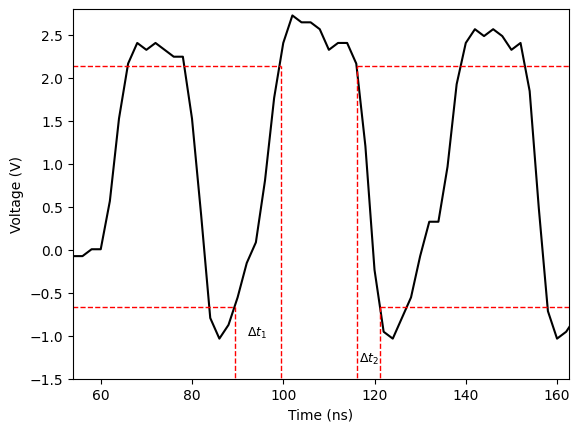
\includegraphics[width=1\columnwidth]{images/risefall.png}
    \caption{Rise and fall times calculated from 10\% to 90\% marks ($\Delta t_1$ and $\Delta t_2$ respectively) for the JK output Q}
\end{figure}

\begin{figure}[H]
    \centering
    \begin{subfigure}[b]{0.5\textwidth}
        \centering
        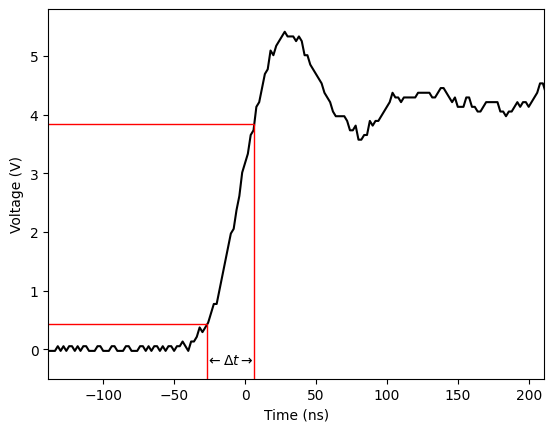
\includegraphics[width=\textwidth]{images/rise.png}
        \caption{}
    \end{subfigure}
    \hfill
    \begin{subfigure}[b]{0.5\textwidth}
        \centering
        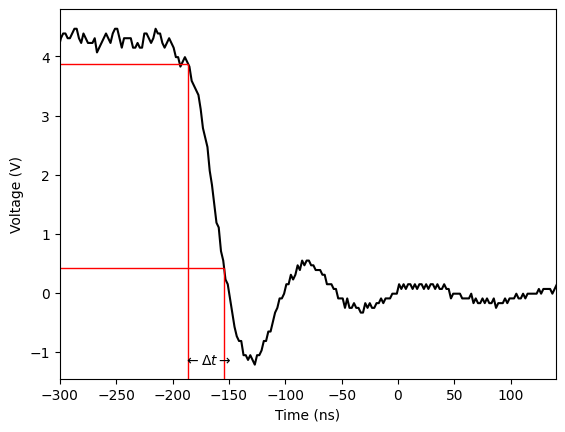
\includegraphics[width=\textwidth]{images/fall.png}
        \caption{}
    \end{subfigure}
    \hfill
    \caption{Plots depicting (a) rise time and (b) fall time of the clock signal}
\end{figure}

The rise and fall time of the clock signal came out to be almost equal at 32.9 ns and 31.8 ns respectively.
Similarly, the rise and fall time of the JK output (Q) came out to be 10.15 ns and 5.11 ns. Here, the rise time is almost double the fall time.

\subsection*{Racing Condition}

From the fig. \ref{race-plot}, one can calculate the average time period of the toggling output as,

\begin{align*}
    T_\text{toggle} &= 36.1 \text{ ns}\\
    \implies f_\text{toggle} &= 27.7 \text{ MHz}
\end{align*}

\begin{figure}[H]
    \centering
    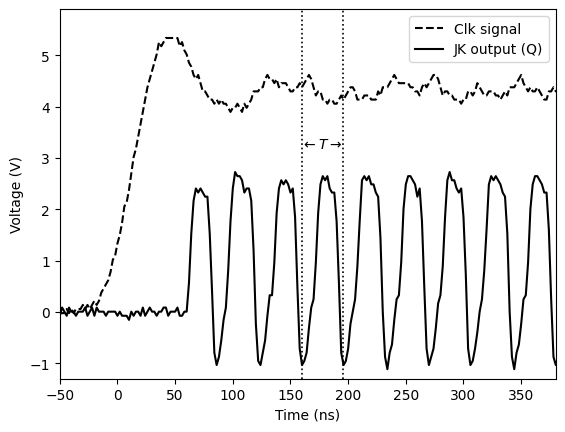
\includegraphics[width=0.95\columnwidth]{images/racing.png}
    \caption{Race-around condition depicted for the output Q once the clock goes high. $T$ refers to the time period between successive toggles.}
    \label{race-plot}
\end{figure}


The high frequency ($\sim 10^7$ Hz) explains why one cannot observe racing condition by just observing the output through an LED.

\subsection*{Propagation Delay}

\begin{figure}[H]
    \centering
    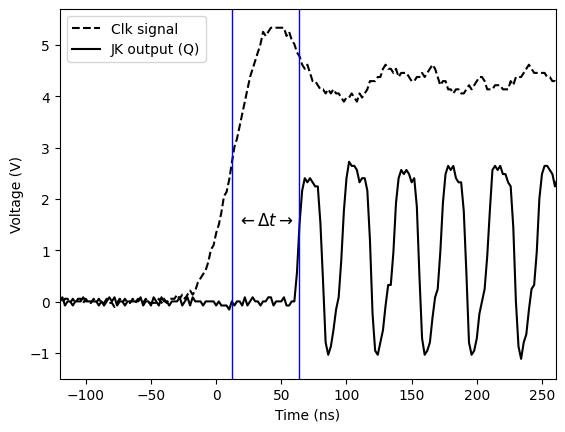
\includegraphics[width=1\columnwidth]{images/propagation.png}
    \caption{Propagation delay depicted between the clock signal and the output Q as $\Delta t$}
\end{figure}

The propagation delay of the flip-flop is measured from the 50\% rise mark of the clock signal to 50\% that of the JK output (Q). This value came about to be around 51.2 ns.\\

As mentioned earlier, one of the ways to avoid the racing condition was to make the propagation delay ($\Delta t$) greater than the duration of the clock pulse ($T$), hence $T < 51.2$ ns, or the frequency of the clock pulse should be $f > 27.7$ MHz.\\
% \newpage